\documentclass[a4paper,12pt]{article}
\usepackage{amsmath}
\usepackage{amssymb}
\usepackage[utf8]{inputenc}
\usepackage[T1]{fontenc}
\usepackage{lmodern}
\usepackage{indentfirst}
\usepackage{geometry}
\usepackage{array}
\usepackage[pdftex]{color,graphicx}
\usepackage{subfigure}
\usepackage{afterpage}
\usepackage{setspace}
\usepackage{color}
\usepackage{wrapfig}
\usepackage{listings} 
\usepackage{datetime}
\usepackage{epstopdf}
\usepackage{hyperref}

\renewcommand{\onehalfspacing}{\setstretch{1.6}}

\geometry{tmargin=2.5cm,bmargin=2.5cm,lmargin=2.5cm,rmargin=2.5cm}
\setlength{\parindent}{1cm}
\setlength{\parskip}{0mm}

\newenvironment{lista}{
\begin{itemize}
  \setlength{\itemsep}{1pt}
  \setlength{\parskip}{0pt}
  \setlength{\parsep}{0pt}
}{\end{itemize}}

\newcommand{\linia}{\rule{\linewidth}{0.4mm}}

\definecolor{lbcolor}{rgb}{0.95,0.95,0.95}
\lstset{
  backgroundcolor=\color{lbcolor},
  tabsize=4,
  language=C++,
  captionpos=b,
  tabsize=3,
  frame=lines,
  numbers=left,
  numberstyle=\tiny,
  numbersep=5pt,
  breaklines=true,
  showstringspaces=false,
  basicstyle=\footnotesize,
  identifierstyle=\color{magenta},
  keywordstyle=\color[rgb]{0,0,1},
  commentstyle=\color{green},
  stringstyle=\color{red}
  }

\begin{document}

\noindent
\begin{tabular}{|c|p{11cm}|c|} \hline 
Michał Szczygieł & Aleksander Śmierciak & \ddmmyyyydate\today \tabularnewline
\hline 
\end{tabular}


\section*{Zadanie 7 - Test Millera-Rabina - MPI}

Zadanie miało na celu implementację programu określającego dla każdej liczby w ciągu danych wejściowych czy jest ona liczbą pierwszą czy też złożoną. Wykorzystać w tym celu miano test pierwszości liczb Rabina-Millera, a sam program napisać w oparciu o architekturę MPI, umożliwiającą zrównoleglenie potrzebnych obliczeń.
\\

Aby zrealizować schemat komunikacyjny z polecenia (scentralizowana struktura), należało wykorzystać \emph{MPI\_Send} oraz \emph{MPI\_Recv} – blokujące funkcje wymiany danych między procesami. \\

Pseudokod dla rozwiązania odpowiadającego schematowi z polecenia prezentuje się następująco:
\begin{lista}
\item dla każdej liczby wyznacz identyfikator węzła obliczającego
\item jeśli węzeł jest węzłem głównym wyślij liczbę do wybranego węzła obliczającego
\item jeśli nie, ale węzeł jest węzłem obliczającym  sprawdź czy liczba jest liczbą pierwszą
\item jeśli węzeł jest węzłem głównym odbierz sprawdzone liczby od węzła obliczającego
\end{lista}

Faktyczny kod źródłowy temu odpowiadający znajduje się w pliku main.cpp, w funkcji searchForPrimesUsingMPI().\\

\begin{lstlisting}
void searchForPrimes(const string &inputPath, const unsigned int repeatCount)
{
LongMultimap results;
const LongVector *numbers = readNumbersFromFile(inputPath);

searchForPrimesUsingMPI(numbers, results, repeatCount);

delete numbers;
}
\end{lstlisting}


\begin{center}
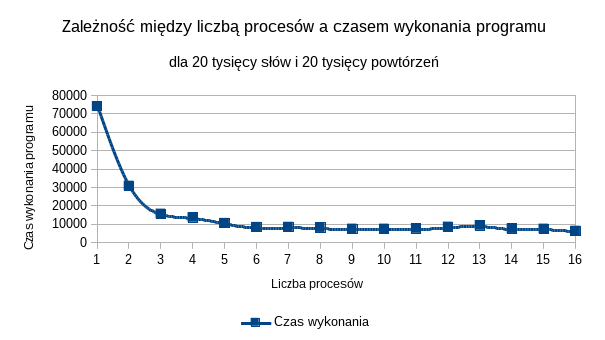
\includegraphics[width=0.7\textwidth]{data/wykonanieProgramu.png}
\end{center}

Patrząc na wykresy wydajności tak napisanej implementacji należy mieć na uwadze, że jeden proces zawsze zajmował się jedynie wysyłaniem danych wejściowych i zapisywaniem danych wyjściowych – nie brał udziału w samych obliczeniach. Bezpośrednio wynika z takiego ograniczenia niemożność uruchomienia programu dla liczby procesów równej 1; w celu przedstawienia wydajności „dla 1 procesu” napisano osobny program, sekwencyjnie sprawdzający liczby po kolei. \\

Z uwagi na specyfikę komputera, na którym były wykonywane obliczenia (12-rdzeniowy procesor), zauważalne przyspieszenie obserwować można do 12 procesów włącznie.

\begin{center}
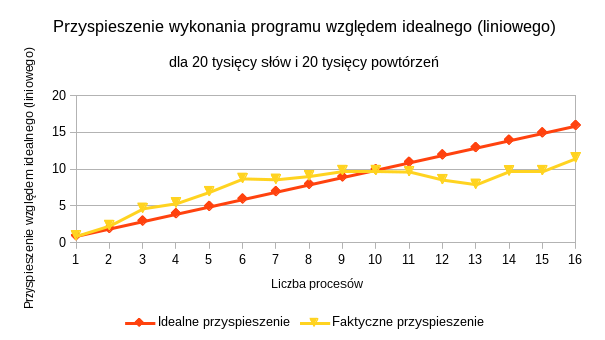
\includegraphics[width=0.7\textwidth]{data/przyspieszenie.png}
\end{center}

\section*{Wnioski}
Środowisko MPI jest w naszym mniemaniu znacznie mniej wygodne dla komunikacji międzyprocesowej przy dokonywaniu zaawansowanych obliczeń równoległych. Wynika to ze sposobu zapisu tej komunikacji, dla żadnego z popularnych języków programowania niebędącego "natywnym", niejednokrotnych ograniczeń dotyczących typów zmiennych i sposobu ich przekazywania (wspomniany w kodzie brak typu boolean, "załatany" typem \emph{MPI\_BOOL} dopiero w nowszym standardzie), a także z mniejszej konfigurowalności architektury, którą można przy pomocy tego środowiska stworzyć.

\end{document}